\section*{Problema P9.50}

\renewcommand*\thesection{9.50}
\numberwithin{equation}{section}

\begin{center}
    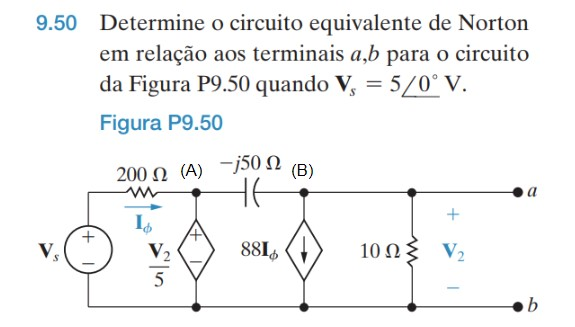
\includegraphics[scale=1.0]{P9.50.jpg}
\end{center}

Em um circuito equivalente norton, temos

\[ I_N = I_{SC} \quad, \quad R_N = R_{th}  \]

Vamos começar calculando a tensão de Thevenin \(V_{th}\) entre os terminais \(a\) e \(b\), abrindo-os.

Expressando as variáveis de controle em função dos elementos do circuito, obtemos

\begin{equation}\label{eq:9.50.1}
    V_{2} = V_B
\end{equation}

\begin{equation}\label{eq:9.50.2}
    I_{\phi} = \frac{5V - V_A}{200 \;\Omega}
\end{equation}

Feito isso, aplicamos análise nodal dos nós essenciais \( A \) e \( B \).
Começamos pelo nó \( A \). Obtemos de imediato que

\begin{equation}\label{eq:9.50.3}
    V_{A} = \frac{V_2}{5} = \frac{V_B}{5}
\end{equation}

Agora vamos para o nó \( B \).

\[ \frac{V_B - V_A}{-j50 \;\Omega} + 88I_{\phi} + \frac{V_B - 0}{10 \;\Omega} = 0 \]

Usando (\ref{eq:9.50.2}) e (\ref{eq:9.50.3}), temos

\[ \frac{V_B - \frac{V_B}{5}}{-j50 \;\Omega} + 88\frac{5V - \frac{V_B}{5}}{200 \;\Omega} + \frac{V_B}{10 \;\Omega} = 0 \]

Isolando \( V_{B} \), temos

\[ \frac{V_B}{-j50} - \frac{V_B}{-j250} - \frac{88V_B}{1000} + \frac{V_B}{10} = - 2.2\]

\[ V_B = - \frac{2.2}{\frac{1}{-j50} - \frac{1}{-j250} - \frac{88}{1000} + \frac{1}{10}}\]

\begin{equation}\label{eq:9.50.4}
    V_{B} = - 66 + j88 V = 110\fase{126.86} V
\end{equation}

Usando (\ref{eq:9.50.3}), obtemos

\begin{equation}\label{eq:9.50.5}
    V_{A} = 22\fase{126.86} V
\end{equation}

Assim, obtemos que a tensão de Thevenin é dada por

\begin{equation}\label{eq:9.50.6}
    V_{th} = V_{ab} = V_B = 110\fase{126.86} V
\end{equation}

Agora calculamos a corrente de curto-circuito \( I_{sc}\). 
Curto circuitamos os terminais \( a \) e \( b \), e novamente expressamos as variáveis de controle em função dos elementos
do circuito.

\begin{equation}\label{eq:9.50.7}
    V_{2} = 0 V
\end{equation}

\begin{equation}\label{eq:9.50.8}
    I_{\phi} = \frac{5V - V_A}{200 \;\Omega}
\end{equation}

Agora aplicamos análise nodal nos nós essencias \(A\) e \( B \).
De imediato temos que

\[ V_{A} = \frac{V_2}{5} = \frac{V_B}{5} \]

No entanto, devido ao curto-circuito, observe que 

\[ V_B = 0V \]

E portanto,

\[ V_A = V_B = 0V \]

Escrevendo a equação de nó de \(B\), temos

\[ \frac{V_B - \frac{V_B}{5}}{-j50 \;\Omega} + 88\frac{5V - \frac{V_B}{5}}{200 \;\Omega} + I_{sc} = 0 \]

Substituindo e isolando  \(I_{sc}\),

\[ 0 + 88\frac{5V}{200 \;\Omega} + I_{sc} = 0 \]

\begin{equation}\label{eq:9.50.9}
    I_{sc} = - 2.2 \un{A} = 2.2\fase{180} \un{A}
\end{equation}

Usando (\ref{eq:9.50.9}) e (\ref{eq:9.50.6}), obtemos a resistência de Thevenin \( R_{th} \).

\begin{equation}\label{eq:9.50.10}
    R_{th} = \frac{V_{th}}{I_{sc}} = \frac{110\fase{126.86}}{2.2\fase{180}} = 50\fase{-53.14} \Omega
\end{equation}

Finalmente,

\[ \boxed{R_{N} = 50\fase{-53.14} \Omega = 30 - j40 \Omega}  \]

\[ \boxed{I_{N} = - 2.2 \un{A}}  \]








